\section{Per-search alignment options}
\label{sec:appendix-search-options}

The third argument of \texttt{mmsearch} accepts a
\texttt{bioseq\_aligner\_options} composite value, rather than a JSON object.
It changes settings for
that search without changing the session GUCs. The two SQL overloads accept
\texttt{(target, query)} and \texttt{(target, query, options)}. Both sequence
arguments have type \texttt{bioseq.seq}. The same options form applies to
a stored-column search with a constant query and to a supported sequence join.
The predicate must belong to a BioSeqDB scan or join. A standalone Boolean
call is not a general scalar alignment function.

The constructor \texttt{aligner\_options} and the composite type occupy the
extension's installation schema. Examples below assume \texttt{public}.
Use the installation schema instead when the extension was installed
elsewhere. The sequence type remains in schema \texttt{bioseq}.

\subsection{Construction, NULL values, and precedence}
\label{sec:appendix-options-precedence}

All 36 constructor arguments default to NULL. Named arguments let a call
change only the fields it needs. Positional arguments follow the field order
in Table~\ref{tab:appendix-options-fields}. Named arguments can also follow
positional arguments.

\par\noindent\begin{minipage}{\linewidth}
\begin{lstlisting}[style=bioseq-appendix-sql,
  caption={Construct and inspect an options value.},
  label={lst:appendix-options-construction}]
SELECT (public.aligner_options(
    kmer_size => 11, window_size => 5)).*;

-- The same two fields, using a positional first argument.
SELECT public.aligner_options(11, window_size => 5);

-- NULL is explicitly typed when used as the whole options value.
SELECT NULL::public.bioseq_aligner_options;
\end{lstlisting}
\end{minipage}

The constructor stores the supplied values. It does not fill omitted fields
with the current GUC values. The search resolves them as follows:
\begin{enumerate}
  \item Session settings supply the alignment defaults.
  \item Each non-NULL options field replaces its corresponding value.
    Omitted fields and explicitly NULL fields both retain the defaults.
    Zero and \texttt{false} are explicit values.
  \item The separate \texttt{index\_read\_requirement} policy starts at
    \texttt{allow}. It has no GUC default.
  \item The selected execution route checks compatibility and derives
    required work from the search and its requested results.
\end{enumerate}

Explicit \texttt{vulkan\_enabled => true} also records a prefilter request
in one scan route. This extra meaning is described in
Section~\ref{sec:appendix-options-algorithms}.
Figure~\ref{fig:appendix-options-precedence} shows ordinary field inheritance.

\begin{figure}[htbp]
\centering
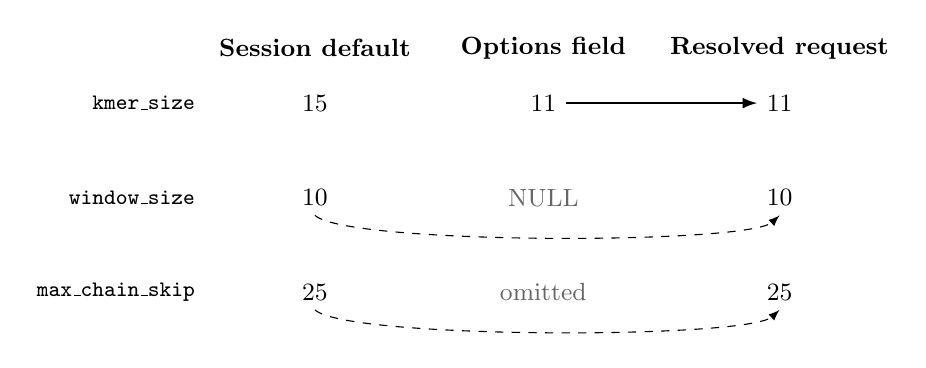
\begin{tikzpicture}[font=\small, >=latex]
  \node[font=\small\bfseries] at (3.9,.7) {Session default};
  \node[font=\small\bfseries] at (6.8,.7) {Options field};
  \node[font=\small\bfseries] at (9.8,.7) {Resolved request};
  \node[anchor=east,font=\footnotesize\ttfamily] at (2.5,0) {kmer\_size};
  \node[anchor=east,font=\footnotesize\ttfamily] at (2.5,-1.2) {window\_size};
  \node[anchor=east,font=\footnotesize\ttfamily] at (2.5,-2.4) {max\_chain\_skip};
  \node (d1) at (3.9,0) {15};
  \node (d2) at (3.9,-1.2) {10};
  \node (d3) at (3.9,-2.4) {25};
  \node (o1) at (6.8,0) {11};
  \node[text=black!60] at (6.8,-1.2) {NULL};
  \node[text=black!60] at (6.8,-2.4) {omitted};
  \node (r1) at (9.8,0) {11};
  \node (r2) at (9.8,-1.2) {10};
  \node (r3) at (9.8,-2.4) {25};
  \draw[->,thick] (o1.east) -- (r1.west);
  \draw[->,dashed] (d2.south)
    .. controls (4.3,-1.8) and (9.4,-1.8) .. (r2.south);
  \draw[->,dashed] (d3.south)
    .. controls (4.3,-3.0) and (9.4,-3.0) .. (r3.south);
\end{tikzpicture}
\caption{A non-NULL field overrides its default. Dashed arrows show
inheritance for NULL and omitted fields. Route checks and parameter
adjustments follow this merge.}
\label{fig:appendix-options-precedence}
\end{figure}

Omitting the third argument, supplying \texttt{public.aligner\_options()},
and supplying \texttt{NULL::public.bioseq\_aligner\_options} all request
the inherited option set. A NULL sequence operand has a different meaning:
it produces no alignment.

Options must become a constant of the exact composite type during planning.
The immutable constructor with constant arguments satisfies this rule.
A typed composite string literal or a constant expression that folds to the
same type is also accepted. A raw composite literal must contain all 36
positions, including empty positions for NULLs. The named constructor is
easier to maintain. Column values, subqueries, volatile wrappers, and
parameters that remain unresolved in a generic prepared plan are unsupported
options expressions.

An ordinary \texttt{BioseqScan} captures the GUC values and overrides in its
plan. A \texttt{BioseqBatchJoin}, including searches with slices or
concatenated sequence arguments,
resolves GUC values again during executor initialization and reapplies the
constant overrides. Changing the relevant alignment GUCs invalidates cached
plans. These routes therefore share the precedence rule while resolving
defaults at different points.

The displayed defaults are requested values. For a short pair, the ordinary
pair adjustment can reduce $k$, $w$, the chain-score threshold, and the seed
threshold when their values equal $15,10,40,3$. Explicitly writing those same
four values does not disable the adjustment. An indexed route must prepare
query sketches compatible with its stored lookup.

\subsection{Complete field reference}
\label{sec:appendix-options-fields}

Every constructor field is nullable. \textbf{I} means SQL \texttt{integer},
\textbf{D} means \texttt{double precision}, and \textbf{B} means
\texttt{boolean}. The four D fields are converted to single precision in
the alignment parameters. In the table, prepend
\texttt{bioseq.aligner.} to each GUC suffix.

\textbf{The numeric intervals below are the corresponding GUC bounds.}
The options constructor and override decoder do not enforce these intervals
for ordinary numeric fields. Algorithm codes and the index-policy code are
checked explicitly. Later kernels impose additional conditions, so even a
value within its GUC interval need not work with every algorithm. Use the
listed intervals together with the route restrictions below.

\begingroup
\footnotesize
\setlength{\tabcolsep}{3pt}
\renewcommand{\arraystretch}{1.12}
\begin{longtable}{@{}>{\raggedright\arraybackslash}p{.27\linewidth}
  >{\raggedright\arraybackslash}p{.69\linewidth}@{}}
\caption{All options fields in composite order. Defaults are initial session
values, except for the independent index policy.}
\label{tab:appendix-options-fields}\\
\toprule
\textbf{Field and type} & \textbf{GUC suffix, default, range, and effect}\\
\midrule
\endfirsthead
\multicolumn{2}{l}{\textit{Search options, continued}}\\
\toprule
\textbf{Field and type} & \textbf{GUC suffix, default, range, and effect}\\
\midrule
\endhead
\midrule
\multicolumn{2}{r}{\textit{Continued on the next page}}\\
\endfoot
\bottomrule
\endlastfoot
\path{kmer_size} (I) &
  \path{minimizer.kmer_size}. Default 15, GUC range $1\ldots64$.
  Length of each $k$-mer in sequence symbols.\\
\path{window_size} (I) &
  \path{minimizer.window_size}. Default 10, GUC range $1\ldots1024$.
  Number of consecutive $k$-mers in a minimizer window.\\
\path{max_gap} (I) &
  \path{chaining.maximum_gap}. Default 5000, GUC range $1\ldots2^{30}$.
  Distance limit used by chaining. The scalar chainer raises it to at least
  the bandwidth.\\
\path{max_gap_ref} (I) &
  \path{chaining.maximum_reference_gap}. Default $-1$, GUC range
  $-1\ldots2^{30}$. Stored reference-gap option, currently unused by
  execution.\\
\path{bandwidth} (I) &
  \path{chaining.bandwidth}. Default 500, GUC range $1\ldots2^{20}$.
  Diagonal-band setting for the algorithms that use it.\\
\path{bandwidth_long} (I) &
  \path{chaining.long_join_bandwidth}. Default 0, GUC range
  $0\ldots2^{20}$. Stored long-join option, currently unused by execution.\\
\path{max_chain_skip} (I) &
  \path{chaining.maximum_skipped_anchors}. Default 25, GUC range
  $0\ldots2^{20}$. Early-stop limit interpreted by the selected chainer.
  SQL SIMD chaining requires a positive value.\\
\path{max_chain_iter} (I) &
  \path{chaining.maximum_predecessors}. Default 5000, GUC range
  $1\ldots2^{22}$. Predecessor-scan limit for scan-based chainers.
  The scalar chainer can inspect one additional candidate. RMQ does not
  use this field.\\
\path{min_seed_count} (I) &
  \path{chaining.minimum_seed_count}. Default 3, GUC range
  $0\ldots2^{20}$. Minimum accepted chain seed count.\\
\path{min_chain_score} (I) &
  \path{chaining.minimum_score}. Default 40, GUC range $0\ldots2^{20}$.
  Minimum accepted chain score.\\
\path{chain_gap_scale} (D) &
  \path{chaining.gap_penalty_scale}. Default 0.8, GUC range $0\ldots100$.
  Scale for the chaining gap penalty.\\
\path{chain_skip_scale} (D) &
  \path{chaining.skip_penalty_scale}. Default 0, GUC range $0\ldots100$.
  Scale for the chaining skip (distance) penalty.\\
\path{mask_level} (D) &
  \path{secondary.overlap_threshold}. Default 0.5, GUC range $0\ldots1$.
  Overlap threshold used when assigning secondary mappings.\\
\path{mask_len} (I) &
  \path{secondary.uncovered_length_limit}. Default $2^{31}-1$,
  GUC range $0\ldots2^{31}-1$. Uncovered-length limit in that assignment.\\
\path{pri_ratio} (D) &
  \path{secondary.score_ratio_threshold}. Default 0.8, GUC range
  $0\ldots1$. Secondary-to-primary score threshold. Zero bypasses this
  secondary filtering step, including its count limit.\\
\path{best_n} (I) &
  \path{secondary.maximum_count}. Default 5, GUC range $0\ldots1024$.
  Maximum secondary alignments kept by the filter, counted together across
  all primary alignments in its input. It is not an SQL result-row limit.\\
\path{match_score} (I) &
  \path{scoring.match_score}. Default 2, GUC range $1\ldots127$.
  Score for a matching base.\\
\path{mismatch_pen} (I) &
  \path{scoring.mismatch_penalty}. Default 4, GUC range $1\ldots127$.
  Penalty for a mismatching base.\\
\path{gap_open1} (I) &
  \path{scoring.short_gap_open_penalty}. Default 4, GUC range
  $0\ldots127$. First gap-opening penalty.\\
\path{gap_ext1} (I) &
  \path{scoring.short_gap_extension_penalty}. Default 2, GUC range
  $0\ldots127$. First gap-extension penalty.\\
\path{gap_open2} (I) &
  \path{scoring.long_gap_open_penalty}. Default 24, GUC range
  $0\ldots127$. Second gap-opening penalty, used by KSW2.\\
\path{gap_ext2} (I) &
  \path{scoring.long_gap_extension_penalty}. Default 1, GUC range
  $0\ldots127$. Second gap-extension penalty, used by KSW2.\\
\path{sc_ambi} (I) &
  \path{scoring.ambiguous_base_penalty}. Default 1, GUC range
  $0\ldots127$. Penalty for ambiguous bases.\\
\path{zdrop} (I) &
  \path{scoring.z_drop_threshold}. Default 400, GUC range
  $-1\ldots2^{20}$. KSW2 Z-drop threshold, or BlockAligner X-drop
  threshold for end extensions.\\
\path{end_bonus} (I) &
  \path{scoring.end_bonus}. Default $-1$, GUC range $-1\ldots2^{20}$.
  KSW2 sequence-end bonus. $-1$ disables the bonus.\\
\path{max_occ} (I) &
  \path{seeding.maximum_occurrence}. Default 500, GUC range
  $1\ldots2^{24}$. Excludes seed keys whose target occurrence count
  exceeds this limit.\\
\path{mid_occ} (I) &
  \path{seeding.intermediate_occurrence_threshold}. Default 500,
  GUC range $1\ldots2^{24}$. Stored intermediate threshold, currently
  unused by execution.\\
\path{block_min_size} (I) &
  \path{block_alignment.minimum_block_size}. Default 32, GUC range
  $8\ldots4096$. Minimum adaptive block size for BlockAligner.\\
\path{block_max_size} (I) &
  \path{block_alignment.maximum_block_size}. Default 256, GUC range
  $8\ldots16384$. Maximum adaptive block size for BlockAligner.\\
\path{chaining_algorithm} (I) &
  \path{chaining.algorithm}. Default 0, accepted codes $0\ldots3$.
  See Table~\ref{tab:appendix-options-algorithms}.\\
\path{base_alignment_algorithm} (I) &
  \path{base_alignment.algorithm}. Default 1, accepted codes $0,1$.
  See Table~\ref{tab:appendix-options-algorithms}.\\
\path{minimizer_algorithm} (I) &
  \path{minimizer.algorithm}. Default 0, accepted codes $0\ldots4$.
  See Table~\ref{tab:appendix-options-algorithms}.\\
\path{vulkan_enabled} (B) &
  \path{vulkan.enabled}. Default \texttt{true}, values
  \texttt{true}/\texttt{false}. Allows Vulkan execution. An explicit true
  value also has the prefilter meaning described below.\\
\path{vulkan_seed_hits_enabled} (B) &
  \path{vulkan.seed_lookup.enabled}. Default \texttt{false}, values
  \texttt{true}/\texttt{false}. Selects Vulkan seed lookup.\\
\path{vulkan_index_cache_enabled} (B) &
  \path{vulkan.index_cache.enabled}. Default \texttt{true}, values
  \texttt{true}/\texttt{false}. Controls caching of GPU index uploads.\\
\path{index_read_requirement} (I) &
  No GUC. Default 0, accepted codes $0\ldots2$.
  Selects the persisted-index policy described below.\\
\end{longtable}
\endgroup

The three stored but unused numeric options remain part of the public
composite. Assigning them currently does not implement a separate reference
gap, a long-join pass, or intermediate occurrence filtering.

\subsection{Algorithm codes and route restrictions}
\label{sec:appendix-options-algorithms}

Algorithm fields use integer codes. Their GUC counterparts use the names in
Table~\ref{tab:appendix-options-algorithms}. A valid code selects a family,
but does not guarantee that the input, hardware, or other choices are
compatible. Sections~\ref{sec:configured-cpu-minimizers} and
\ref{sec:chaining-bioseqdb} explain the algorithm families.

\begin{table}[htbp]
\centering
\footnotesize
\begin{tabularx}{\linewidth}{@{}p{.30\linewidth}rX@{}}
\toprule
\textbf{Options field} & \textbf{Code} & \textbf{GUC value}\\
\midrule
\path{minimizer_algorithm} & 0 & \path{scalar}\\
 & 1 & \path{simd_minimap2_reference}\\
 & 2 & \path{two_stack_nthash}\\
 & 3 & \path{vulkan_minimap_integer}\\
 & 4 & \path{bounded_nthash_simd}\\
\midrule
\path{chaining_algorithm} & 0 & \path{scalar_minimap2}\\
 & 1 & \path{simd_minimap2}\\
 & 2 & \path{range_minimum_query}\\
 & 3 & \path{vulkan_tiled_dynamic_programming}\\
\midrule
\path{base_alignment_algorithm} & 0 & \path{ksw2}\\
 & 1 & \path{block_aligner}\\
\bottomrule
\end{tabularx}
\caption{Integer options codes and their named GUC equivalents.}
\label{tab:appendix-options-algorithms}
\end{table}

Keep the following restrictions in mind:
\begin{itemize}
  \item Bounded ntHash SIMD requires DNA4, $k=15$, and $w=10$.
    SQL SIMD chaining uses the bounded policy and requires positive
    \texttt{max\_chain\_skip} and \texttt{max\_chain\_iter}.
    Unsupported SIMD chaining is not retried as scalar chaining.
  \item BlockAligner uses the first gap-penalty pair. Both penalties must
    be positive and their sum must not exceed 128. After widening to at least
    the active lane count, its minimum and maximum block sizes must be
    powers of two with minimum no larger than maximum. End extension
    requires a nonnegative \texttt{zdrop}. Invalid BlockAligner contracts
    can terminate the backend, so arbitrary numeric options should not be
    used to probe its limits.
  \item Biological Vulkan stages require the complete supported execution
    route. The options object exposes only three Vulkan Boolean fields.
    Fused frontend, GPU index build, and GPU alignment extension are
    controlled by separate GUCs. Selecting a Vulkan algorithm code alone
    is insufficient.
  \item In an ordinary scan with an eligible exact edit-distance filter,
    explicit \texttt{vulkan\_enabled => true} requests the standalone
    Vulkan prefilter. Merely inheriting the default enabled GUC does not
    make this request. Consequently, that explicit option and a session
    \texttt{SET} are not always equivalent.
\end{itemize}

The options object does not contain output-stage flags. Requesting CIGAR,
edit distance, divergence, or mapping quality through the SQL result helpers
determines the extra work. Choosing a base aligner alone does not force base
alignment for a coordinate-only search. The internal batched KSW2 route is
not an additional SQL algorithm code.

\subsection{Per-call persisted-index policy}
\label{sec:appendix-options-index-policy}

\begin{description}
  \item[0: \texttt{allow}.] Follow the normal index-reading policy. A
    compatible persisted lookup may be used, and an unavailable or
    inapplicable lookup may be recomputed. This value does not override
    \texttt{bioseq.index.sequence\_read.enabled} to enable index reads.
  \item[1: \texttt{require\_absent}.] Disable persisted target-index reads
    for this search. It does not delete an existing index. Separate
    persistence settings can still allow a recomputed index to be written.
  \item[2: \texttt{require\_compatible\_persisted}.] Require a compatible
    persisted generation. A recomputed target index or a transient assembled
    index in memory does not satisfy the requirement. Reusing a retained
    reader for the compatible persisted generation does satisfy it.
    The current prepared-reader route
    belongs to \texttt{BioseqBatchJoin}. An ordinary executable
    \texttt{BioseqScan} rejects this requirement.
\end{description}

A transformed target, such as a slice or concatenation, must be searched
through its evaluated logical view.
Its route forces \texttt{require\_absent} and rejects code 2. For an
untransformed stored target, compatibility includes its source generation,
alphabet, minimizer scheme, producer, and sketch parameters.

\subsection{Search examples}
\label{sec:appendix-options-examples}

Assume \texttt{refs} and \texttt{queries} are BioSeqDB sequence tables with
an \texttt{id} column and a \texttt{seq} column of type
\texttt{bioseq.seq('dna4',32)}. Listing~\ref{lst:appendix-options-join}
sets a session $k$-mer default of 15, then overrides it to 11 for the join.
The other explicitly selected values apply only to this predicate.

\par\noindent\begin{minipage}{\linewidth}
\begin{lstlisting}[style=bioseq-appendix-sql,
  caption={Override session defaults for a sequence join.},
  label={lst:appendix-options-join}]
BEGIN;
SET LOCAL bioseq.aligner.minimizer.kmer_size = 15;
SELECT r.id, q.id
FROM refs AS r JOIN queries AS q
  ON public.mmsearch(r.seq, q.seq,
       public.aligner_options(
         kmer_size => 11, window_size => 5,
         minimizer_algorithm => 0,
         chaining_algorithm => 0,
         index_read_requirement => 1));
COMMIT;
\end{lstlisting}
\end{minipage}

A constant query uses the same third argument. The short-query example
below explicitly sets sketch and chain thresholds. It requests an alignment
search, not an exact substring test.

\par\noindent\begin{minipage}{\linewidth}
\begin{lstlisting}[style=bioseq-appendix-sql,
  caption={Search stored sequences with a typed constant query.},
  label={lst:appendix-options-constant-query}]
SELECT r.id
FROM refs AS r
WHERE public.mmsearch(
  r.seq,
  'ACGTTGCAAGTCGATCGTACGATGCTAGCTAGGCTAACGT'
    ::bioseq.seq('dna4',32),
  public.aligner_options(
    kmer_size => 7, window_size => 1,
    min_seed_count => 1, min_chain_score => 7,
    minimizer_algorithm => 0, chaining_algorithm => 0,
    index_read_requirement => 1));
\end{lstlisting}
\end{minipage}

To retain every session alignment default while giving the third argument
explicitly, use the typed NULL form:

\par\noindent\begin{minipage}{\linewidth}
\begin{lstlisting}[style=bioseq-appendix-sql,
  caption={Use the three-argument overload without overrides.},
  label={lst:appendix-options-null}]
SELECT r.id, q.id
FROM refs AS r JOIN queries AS q
  ON public.mmsearch(
    r.seq, q.seq, NULL::public.bioseq_aligner_options);
\end{lstlisting}
\end{minipage}
